\chapter{Physical Terminology}

\section{anisotropy}
各向异性或非均向性,指物体的全部或部分属性性质随方向的不同有不同的变化

在计算机图形学中,各向异性表面在围绕几何法线旋转时外观会发生变化。

任何具有细粒度的东西,会产生影响外观的作用。

\subsection{anisotropy reflect}
基于反射表面上存在的小凹槽或凸起,改变光源照射物体的方向,反射在各个方向上具有不同的特性。

可用来平滑图像,克服高斯模糊的缺陷。

\subsection{isotropy reflect}
表面反射均匀具有模糊效果, 反射总是在与颗粒相反的方向拉伸。

\section{Light}

\subsection{Conception}

\subsubsection{Absorption \& Scattering}

吸收与散射, 当光在一个不均匀介质中或半透明的材质中传播时,会被吸收或散射。

\subsection{Refraction}

\subsubsection{IOR}
index of refraction,折射率,光在真空中的传播速度与光在介质中的传播速度之比。
折射率与介质的电磁性有关,

\paragraph{绝对折射率}

光在某种介质中的速度为v,真空中的光速为c,则介质的绝对折射率为$n=\frac{c}{v}$

\paragraph{相对折射率}

光从介质1射入介质2发生折射时,入射角$\theta_{1}$与折射角$\theta_{2}$的正弦之比$n_{21}$
叫做介质2相对介质1的折射率。
\begin{align*}
    n_{1} \cdot sin(\theta_{1}) &= n_{2} \cdot sin(\theta_{2}) \\
    n_{21} &= \frac{n_{2}}{n_{1}}
\end{align*}

\paragraph{全反射}

光由相对光密介质射入相对光疏介质,且入射角大于等于临界角C。临界角是指入射角满足折射角为$90^{\circ}$。
\begin{align*}
    \frac{n_{1}}{n_{2}} = \frac{sin90^{\circ}}{sinC}
\end{align*}
空气的折射率是$n_{2}=1$, 则介质向空气入射可简化为$n=1/sinC$.

\paragraph{光色散}

对不同的波长,介质的折射率$n(\lambda)$不同,这叫做光色散.

\subsection{Reflectance}

反射率,是用来衡量物质反射能力的量,定义为物体表面反射能量与达到物体表面入射能量的比率。反射率是波长的函数,
指某段波长向一定方向的反射,不同波长就有不同的反射率。
\begin{align*}
    \phi(\lambda) = \frac{E_{R}(\lambda)}{E_{I}(\lambda)} = \frac{\pi L(\lambda)}{E_{I}(\lambda)}
\end{align*}

\subsection{Albedo}

反照率,指地表在太阳辐射的影响下,反射辐射通量与入射辐射通量的比值。albedo是对全波段的,是反射率在所有方向上的积分。

\begin{align*}
    \alpha = \frac{M}{E}
\end{align*}

\subsubsection{White Sky Albedo}

WSA,白空反照率,指忽略太阳直射辐射,只考虑地物对大气散射辐射的反射情况。

\subsubsection{Black Sky Albedo}

BSA,黑空反照率。指忽略大气散射,只考虑地物对太阳直射,入射,辐射的反射情况

\subsubsection{Blue Sky Albedo}

地物真实反照率,又称为蓝空反照率,或半球-半球反射率BHR

\begin{align*}
    BHR \approx (1-s)WSA + sBSA 
\end{align*}

其中s是天空散射光比例。

\subsection{辐射学}

\begin{center}
    \begin{tabular}{|c|c|c|c|c|} \hline
       \hbox{名称} & \hbox{单位} & \hbox{符号} & \hbox{对应色度单位} & \hbox{色度单位} \\ \hline
       \hbox{Radiant energy/辐射能} & \hbox{焦耳Q} & \hbox{Q} & \hbox{Luminous energy光能量}  & \hbox{tblbot} \\ \hline
       \hbox{Radiant flux辐通量} & \hbox{瓦特W} & \hbox{$\Phi$} & \hbox{Luminous flux光通量}  & \hbox{流明lm} \\ \hline
       \hbox{Intensity/辐强度} & \hbox{W/sr} & \hbox{I} & \hbox{Luminous intensity光出射度}  & \hbox{坎德拉cd=lm/sr} \\ \hline
       \hbox{Irradiance辐照度} & \hbox{$W/m^{2}$} & \hbox{E} & \hbox{Illuminance发光强度}  & \hbox{勒克斯$lx=lm/m^{2}$} \\ \hline
       \hbox{Radiance辐亮度} & \hbox{$W/(m^{2}sr)$} & \hbox{L} & \hbox{Luminance光亮度}  & \hbox{尼特$nit=lm/(m^{2}sr)$} \\ \hline
    \end{tabular}
\end{center}

\paragraph{辐射能}
energy,$Q_{e}$单位是焦耳$J$,单个光子的辐射能表示为$Q=\frac{nc}{\lambda}$

\paragraph{辐通量}
flux, $\Phi_{e}$,单位时间内发射,接收或传输的能量$\Phi_{e}=\frac{dQ}{dt}$,单位是瓦特W.

\paragraph{辐照度}
irradiance辐照度$E_{e}$, radiant exitance辐出度$M_{e}$,辐照度表示单位面积受到的辐通量$E_{e}=\frac{d\Phi}{dA}$, 
辐出度表示单位面积发出的辐通量$M_{e}=\frac{d\Phi}{dA}$,单位都是$W/m^{2}$,辐通量为$\Phi$的点光源在距离r处球面上的辐照度
为$E_{e}=\frac{\Phi}{4 \pi r^{2}}$.

\paragraph{辐强度}
radiant intensity$I_{e}$,元立体角内的辐通量$I_{e}=\frac{d\Phi}{d\Omega}$,单位是$W/sr$

\paragraph{立体角}
solid angle可以看作平面角在球体上的扩展,单位是球面度$sr$,整个球面的总立体角是$4\pi$,半球面的总立体角和是$2\pi$

\paragraph{辐亮度}
radiance, $L_{e}$表示单位面积和单位立体角上的辐通量$L_{e}=\frac{d^{2}\Phi_{e}}{dA^{T}d\Omega}=\frac{d^{2}\Phi_{e}}{cos\theta dA d\Omega}$,
单位是$W/(m^{2}\dot sr)$,辐亮度是用来描述传感器(摄影机,人眼等)感受辐射最常用的量,也是最重要的量。

\paragraph{辐亮度}
它的定义为
\begin{align*}
    L = \frac{d\phi}{dwdA^{\perp}} = \frac{d\pi}{dwdAcos(\theta)}
\end{align*}
其中分母的面积是一个投影面积。那为什么要使用辐亮度这个单位呢?
\begin{itemize}
    \item {符合光的传播特征,光是发散式传播的,辐亮度是一个不会随距离变化的量}
    \item {符合人眼的观察特征,固定辐亮度的物体,在任何距离观察亮度总是相同的}
\end{itemize}

可以这样来证明:设距离$r_{1}$处的一微元表面,面积为$dA$,辐射度为$L$,人眼瞳孔面积为S,视网膜到瞳孔距离为$r_{2}$.
微元表面上在瞳孔上形成的立体角为
$$dw=\frac{dA}{\pi {r_{1}}^{2}}$$
通过瞳孔的辐通量为
$$d\Phi=dwdLS=\frac{dALS}{\pi {r_{1}}^{2}}$$.
设微元表面在视网膜上成像大小为$dA^{'}$,
已知
$$\frac{{r_{1}}^2}{dA}=\frac{r_{2}^2}{dA^{'}}$$,
得到
$$dA^{'}=\frac{dA{r_{2}}^2}{{r_{1}}^2}$$
微元表面在视网膜上成像产生的辐照度

$$
E=\frac{d\Phi}{dA^{'}}=\frac{dALS}{\pi {r_{1}}^2} \cdot \frac{{r_{1}}^2}{dA{r_{2}}^2}=\frac{LS}{\pi {r_{2}}^2}
$$

所以E不会随着$r_{1}$的变化而变化,在不同的距离观察的亮度是相同的。


\subsection{光度学}

辐射的度量是纯物理的方式来描述的,而人眼只能看到波长在400nm~700nm波长的电磁波,所以要转换为描述人眼感知的光学度量,就是
\textbf{光通量}$\Phi_{v}$,单位流明lm,\textbf{光照度}$E_{v}$,单位勒克斯$lx=\frac{lm}{m^2}$,\textbf{发光强度}$I_{v}$单位坎德拉
$cd=\frac{lm}{sr}$,\textbf{光亮度}$L_{v}$,单位$nit=\frac{cd}{m^2}$.

光在不同的波长上的分布,叫做光谱功率分布spectral power distributions(SPD)。人眼作为一种探测器,输入是辐射量表示的可见光辐射,输出的是感受值的光学量。
它们之间的关系可表示为$\Phi_{v}=683.002(lm/w) \cdot \int_{0}^{\infty}{\bar{y}(\lambda)\Phi_{e,\lambda}(\lambda)d\lambda}$, 其中$\Phi_{e,\lambda}$
是光谱功率分布,单位是$W/nm$;$\bar(y)$是光度函数,没有单位;$\lambda$是波长,单位是nm。

所有渲染公式中用到的都是光度学单位,而描述看到的颜色的最终结果的单位是$cd/m^2$。鉴于点光源和平行光源的不同特性,使用不同的单位来描述的,
点光源用\textbf{发光强度I},单位是cd;而平行光源用\textbf{光照度E},单位是lx。,对点光源S,距离r的光照度为$E=\frac{d\Phi}{dA}=\frac{I}{r^2} \cdot 1sr$.

\section{CIE}

自然界真实的光照有很复杂的SPD,但人眼的颜色感受细胞只有三种,分布是红绿蓝RGB三种,即可以将复杂的光谱功率分布转换为RGB表示。

CIE-RGB标准,指定三原色r(645nm), g(526nm), b(444nm)的光谱映射函数和SPD求内积,将一个任意的SPD表示为三个刺激值。
这种方式得到的值有负值,不便于计算,在CIE-RGB基础上改进为CIX-XYZ,将SPD$s(\lambda)$通过求内积转换成三个刺激值XYZ:

\begin{align*}
    X = \int_{380}^{780}s(\lambda)\bar{x}(\lambda)d\lambda, \newline
    Y = \int_{380}^{780}s(\lambda)\bar{y}(\lambda)d\lambda, \newline
    Z = \int_{380}^{780}s(\lambda)\bar{z}(\lambda)d\lambda
\end{align*}

其中$\bar{y}(\lambda)$的曲线就是计算光度学量的光度函数,即Y值可以作为颜色的亮度值。

为了把颜色的亮度和色度区分开,定义

\begin{align*}
    x = \frac{X}{X+Y+Z}, \newline
    y = \frac{Y}{X+Y+Z}, \newline
    z = \frac{Z}{X+Y+Z} = 1 -x - y
\end{align*}

利用上面公式,用xy的值绘制成一张图,得到CIE色品图,是1931 Color Space。图中范围就是人眼可见光范围,
边缘的曲线表示纯色,对应着光谱值,中心点代表D65纯白色。在图中任意取一颜色点,与中心点的延长线交于曲线处的
颜色叫做\textbf{色相hue},中心点与颜色点的距离与中心点延长交于曲线的距离的比值叫\textbf{饱和度saturation}。
从色品图中取一个颜色点,加上亮度值,就构成CIE-XYZ坐标系统来描述任意颜色。

\begin{figure}[h]
    \centering
    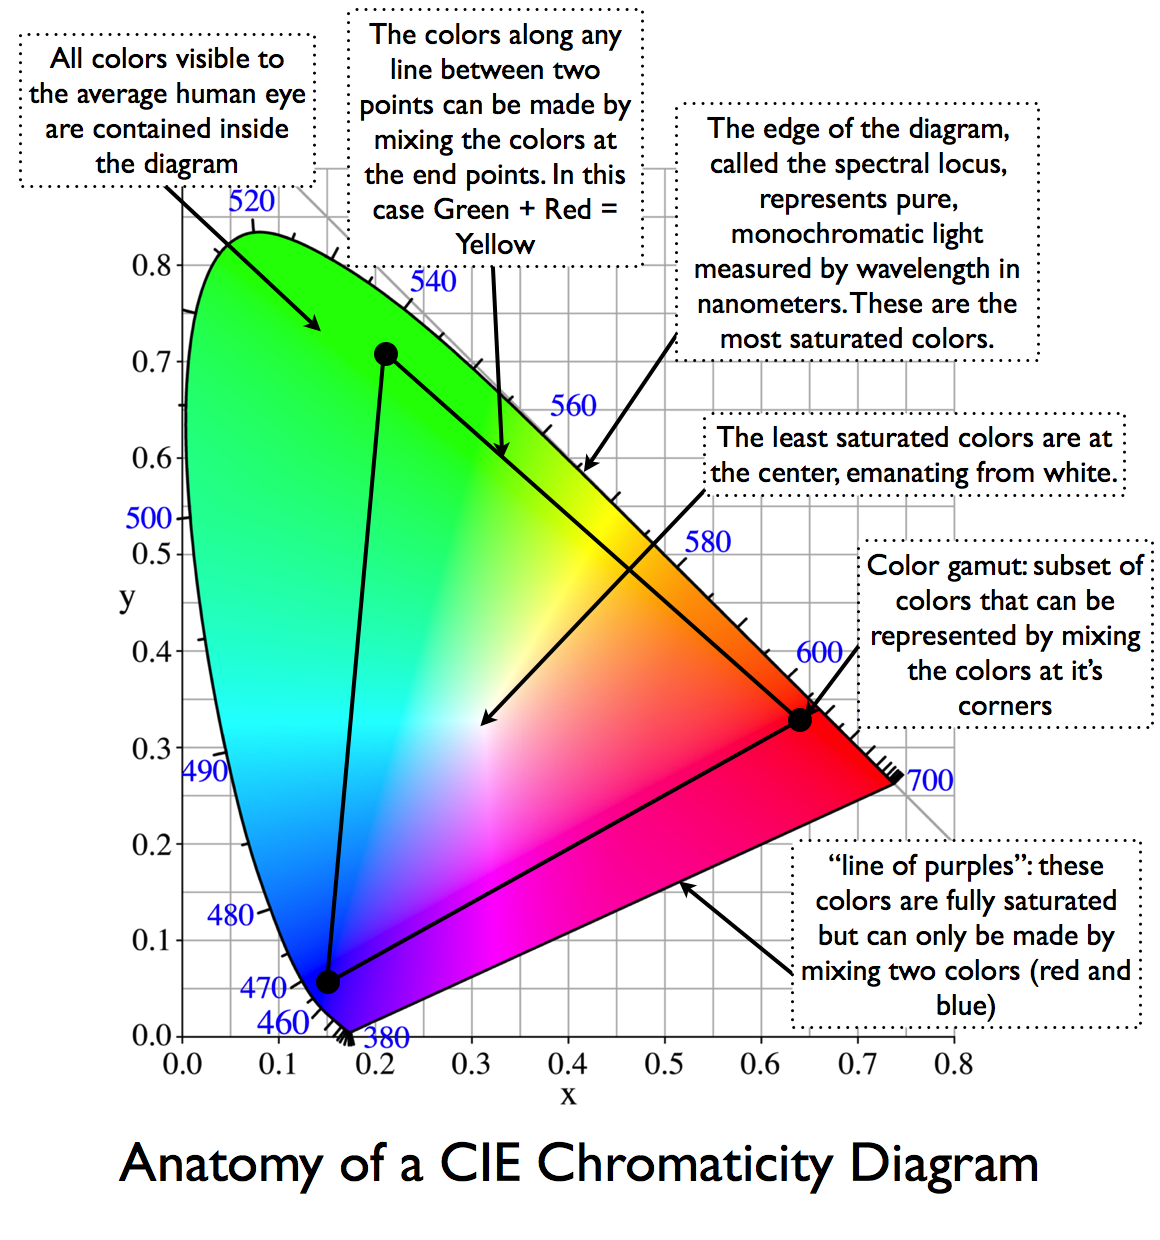
\includegraphics[width=1\textwidth]{images/anatomy-of-a-cie-1931-color-space.png}
\end{figure}

选取三个点作为纯色RGB颜色,形成一个三角形\textbf{色域gamunt},色域中的颜色可以任意进行线性混合。RGB色域有很多种,
,图中三个黑色点就是sRGB色域,还有Adobe 1998色域;DCI-P3苹果系列产品使用的色域;ACEScg一种设计用来计算渲染的色域。
\textbf{色品图中的色域只是一个投影,真实的色域应该是一个立体形的,包括亮度值}。

从RGB色域到XYZ三刺激值的互相转换是线性的,可以用矩阵来表示。如sRGB色域中,有$Y = 0.2126R + 0.7156G + 0.0722B$,Y就是
亮度值,在实时渲染中常用来计算亮度来模拟自动曝光的一个参数。RGB色域并不真实反映物体对光SPD的反馈,但除少数工业级电影的离线渲染
使用频谱渲染,其他都可以满足要求了。

\subsection{伽马校正}

早期的CRT显示器的输入电压和显示亮度并不是线性关系,是$I=V^{2.2}$的非线性关系,显示器的显示亮度和输入值的关系称为
\textbf{EOTF(electrical optical transfer function)},由硬件层实现自动转换。

实时渲染中的颜色值计算都是在线性空间中,为了让显示器正确显示颜色,需要在Framebuffer中进行伽马校正,来抵消EOTF的效果。

人眼对亮度的感受会随着亮度的增高而减弱,如果是线性编码,人眼对低亮度的变化更加敏感,如果使用8bit(0~255)的线性编码颜色,
就会产生很严重的色差。对线性的sRGB进行一次伽马校正后,这样就可以直角显示了,目前大部分图片的格式都经过sRGB伽马校正了。

可是渲染时,从图片中获取的像素值是经过伽马校正的,需要转换为线性空间的sRGB,以便于渲染计算的正确性。最后在FrameBuffer阶段
还是需要进行伽马校正的来保证显示器正确显示最终的色值。

\subsection{HDR - Tone Mapping}
hight dynamic range在渲染和硬件中的两种意思,这里指渲染的意思。

随着PBR渲染及硬件的发展,渲染计算中的光照值的范围需要转换成显示器中的显示范围,这个映射的过程叫做\textbf{Tone Mapping}。
尽可能还原图像的细节,而不仅仅线性的缩放,tone mapping映射为曲线时能保留亮部和暗部的细节。

\subsection{EV100}

计算图像的整体平均亮度是必须的,一般采用log平均的方式

\begin{itemize}
    \item {传统方式是算出图像的亮度log值后,不断DownSample直到一个1x1的texture,即可算出图像的平均亮度}
    \item {现代使用Computer Shader,统计每个亮度范围的像素点数,再综合计算得到一个亮度值}
\end{itemize}

EV(exposure value)在摄影中表示需要曝光值,EV100表示在ISO100标准下的EV值和光亮度的关系,$EV_{100}=log_{2}(\frac{E}{0.78} \cdot q)$
,$q$表示光在光学系统中传递时的损耗,游戏引擎中是一个模拟值,取$q=0.65$。

\chapter{Physical Simulation}

\section{Material Point Method}

物质点法,是一种模拟连续介质的方法,最早被Sulkey等人在1995年发明。
与有限元相比,可以把MPM里面的grid nodes对应到FEM中的DOFs,
把MPM里面的particles对应到FEM中的quadrature points。和FEM里使用显式网格策略
不同,作为一种Element-Free Galerkin(EFG)方法,MPM里面并没有显式的Elements
和Lagrangian grid,只有能够随意移动的粒子,作为quadrature points。这样的特性
非常适合处理大形变,而其背景网格带来的自动碰撞处理,多材料耦合等。由于离散化
出自weak form,使得MPM的physical accuracy有了保证。

\subsection{Moving Least Squares Material Point Method}

移动最小二乘物质点法,

\chapter{Physically Based Rendering}

Physically Based Rendering Toolkit是一个基于物理渲染的开源离线渲染器, 可参考配套的书\cite{PBR3ed}。



\paragraph{Markov Process}

Markov Chain可应用到渲染上是基于Detailed Balance的方法。

光线传递的随机性(光子抵达物体表面材质后被吸收或随机反射)仅由当前状态决定,和历史无关,满足马可夫过程定义。

在渲染中使用Markov Chain Monte Carlo没有复杂的物理,现代所有光线传播的模拟都是基于对渲染方程rendering equation
的求解,而渲染方程已经将原本的物理系统大大的简化了,所以光线传递的物理到底是不是平稳马尔可夫过程和渲染没有任何关系,
渲染只是要计算一个定义域纬度很高的函数而已,对于一个场景,固定的一组输入是会返回一个固定的值,没有什么随机和模糊的东西,
最极端简化就是一个一维函数,Metropolis Sampling的牛逼之处在于它不需要求解函数的积分或者算它的概率分布就能给你提供一系列
和目标高数概率分布一致的样本,这一点对基于Monte Carlo的渲染来说十分重要,叫做重要性采样Importance Sampling。

所以Metropolis Sampling主要用来渲染一些采样路径特别复杂的场景,一般室外大太阳的场景用不着付出额外的计算。Metropolis Light Transport
的论文就是用了一个光源在一个微微打开的门缝后面的场景当例子。

\section{BRDF}

计算整个半球面上的辐照度E
$$
E(p)=\int_{\Omega}L_{i}(p,{\omega}_{i})cos{\theta}_{i}d{\omega}_{i}
$$
把整个辐照度看作是半球上的辐亮度积分,可得
$$
dE(p,{\omega}_{i})=L_{i}(p,{\omega}_{i})cos{\theta}_{i}d{\omega}_{i}
$$
在任意方向上出射的光的辐亮度微分和任意方向上入射光辐亮度微分成正比的
$$
dL_{o}(p,{\omega}_{o}) \propto dE(p,{\omega}_{i}) 
$$
这个比例就是关于${\omega}_{i}$和${\omega}_{o}) $的BRDF函数,记为
$$
f_{r}(p,{\omega}_{o},{\omega}_{i})
=\frac{dL_{o}(p,{\omega}_{o})}{dE(p,{\omega}_{i})}
=\frac{dL_{o}(p,{\omega}_{o})}{L_{i}(p,{\omega}_{i})cos{\theta}_{i}d{\omega}_{i}}
$$
需要注意的是这两个微分的不同,$dL_{o}$是关于值的微分$dE$是在立体角上的微分.

BRDF函数乘以辐照度值,得到的是辐亮度,使单位发生了变化,在整个半球面上积分变成
$$
dL_{o}(p,{\omega}_{o})=\int_{\Omega}f_{r}(p,{\omega}_{o},{\omega}_{i})L_{i}(p,{\omega}_{i})cos{\theta}_{i}d{\omega}_{i}
$$
BRDF满足
\begin{itemize}
    \item {交换律:$f_{r}(p,{\omega}_{i},{\omega}_{o})=f_{r}(p,{\omega}_{o},{\omega}_{i})$}
    \item {能量守恒: $\int_{\Omega}L_{i}(p,{\omega}_{i})cos{\theta}_{i}d{\omega}_{i} \leq 1$}
\end{itemize}

\section{菲涅尔反射}
菲涅尔反射描述一个完全平坦的,由两个不同折射率介质组成的表面对光的反射率。在不同折射率的介质相交平面,光会部分
反射且部分折射,反射的比例就是菲涅尔系数,$0 \leq F_{r} \leq 1$,菲涅尔系数是可以由麦克斯韦方程组直接推导出来的。

已知两种介质的折射率分别为${\eta}_{i}sin{\theta}_{i}={\eta}_{t}sin{\theta}_{t}$,然后根据麦克斯韦方程组计算推导,
平行和垂直偏振光的菲尼尔反射公式
\begin{equation}
    \begin{aligned}
        r_{\parallel}=\frac{{\eta}_{t}sin{\theta}_{i} - {\eta}_{i}sin{\theta}_{t}}{ {\eta}_{t}sin{\theta}_{i} + {\eta}_{i}sin{\theta}_{t}} \\
        r_{\perp}=\frac{{\eta}_{i}sin{\theta}_{i} - {\eta}_{t}sin{\theta}_{t}}{ {\eta}_{i}sin{\theta}_{i} + {\eta}_{t}sin{\theta}_{t}}                
    \end{aligned}
\end{equation}
渲染中使用的是非偏振光,得到
$$
F_{r}=\frac{1}{2}({r_{\parallel}^2}+{r_{\perp}}^2)
$$
在观察角接近掠夺角(90度)的时候,菲涅尔系数趋近于1,这种现象叫做菲涅尔现象。

\paragraph{电介质}
电介质的菲涅尔系数基本上不会随着波长变化,用Schlick近似来表示菲涅尔系数,将观察角为0时菲涅尔系数记为$F_{0}$,
两种介质的折射率比例记为$n$,得到
$$
F_{0}=(\frac{n+1}{n-1})^2
$$
则Schlick近似为
$$
F_{r} \approx F_{0} + (1-F_{0})(1 - cos{\theta}_{i})^5
$$
一般电介质的$F_{0}$值一般都很小,在实时渲染中,直接取0.04作为默认值。

这里说的菲涅尔项是反射的比例,没有反射的部分自然是形成折射,因为这里考虑的是不透明表面光,折射部分的光传入介质内部后,
部分被吸收,部分再次出射形成漫反射/次表面散射。

\paragraph{金属}

相比电介质,差别有几点
\begin{itemize}
    \item {金属内部是可以自由运动电子,折射部分直接被金属吸收了,即金属不会产生漫反射}
    \item {金属的折射率是复数,为$\hat{\eta}=\eta+ik$,k表示吸收率}
    \item {金属的折射率随光波长变化剧烈,因此Schilick近似时要把$F_{0}$用RGB三个分量来表示,电介质的颜色来自漫反射,金属颜色则来自菲涅尔反射或镜面反射}
\end{itemize}

\section{镜面反射项}
对全镜面反射来说,只需要考虑菲涅尔反射的系数,
$$
L_{o}({\omega}_{o})=F_{r}({\omega}_{r})L_{i}({\omega}_{r}=\int_{\Omega}f_{r}({\omega}_{o},{\omega}_{i})L_{i}({\omega}_{i})cos{\theta}_{i}d{\omega}_{i}
$$
其中${\omega}_{r}$和${\omega}_{o}$是关于表面法线对称的。
在BRDF中$F_{r}$如何描述呢?是使用狄拉克$\delta$函数,其表示为
\begin{equation}
    {\delta}(x)= \left\{ 
    \begin{aligned}        
        \infty, x = 0 \\
        0 , x \neq 0        
    \end{aligned}
    \right.
\end{equation}
\begin{equation}
    \begin{aligned}
        \int_{\infty}^{+\infty} {\delta}(x) = 1 \\ 
        \int_{\infty}^{+\infty}f(x){\delta}(x-x_{0})dx = f(x_{0})
    \end{aligned}    
\end{equation}
将狄拉克函数带入到方程中,得到
\begin{equation}
    \begin{aligned}
        L_{o}=\int_{\Omega}\frac{{\delta}({\omega}_{i}-{\omega}_{r})}{cos{\theta}_{i}}F_{r}({\omega}_{i})cos{\theta}_{i}d{\omega}_{i}=F_{r}({\omega}_{r})L_{i}({\omega}_{r}        
    \end{aligned}    
\end{equation}
得到BRDF的表示为
\begin{equation}
    \begin{aligned}
        f_{r}(p,{\omega}_{o},{\omega}_{i})=F_{r}({\omega}_{r})\frac{{\delta}({\omega}_{i}-{\omega}_{r})}{cos{\theta}_{i}}
    \end{aligned}
\end{equation}

\section{漫反射项}
漫反射的物体表面发出的光,吸收后出射形成的部分,通常使用Labertian模型来描述漫反射,这种模型假设在所有方向观察物体表面
的亮度完全相同。Labertian模型在BRDF中表示为$f_{r}=\frac{c}{\pi}$,其中c叫做反照率或固有色,表示光在介质内部出射部分的比例,
$1-c$表示被介质吸收的比例。

这里解释一下为什么要除以$\pi$,在Labertian漫反射模型下,由能量守恒可知,
$$
\int_{\Omega}f_{r}({\omega}_{o},{\omega}_{'})cos{\theta}d{\omega}_{'}=c
$$
因为假设所有方向的亮度相同,因此$f_{r}$和${\omega}_{o},{\omega}_{'}$是无关的,是一个常数,将$f_{r}$提到外面
$$
f_{r}\int_{\Omega}cos{\theta}d{\omega}_{'}=c
$$
$$
f_{r}\int_{\Omega}cos{\theta}d{\omega}_{'}=f_{r}\int_{0}^{2\pi}d\phi\int_{0}^{2\pi}d{\theta}cos{\theta}=f_{r}\pi=c
$$
$$
f_{r}=\frac{c}{\pi}
$$
BRDF的作用之一是将辐照度值E转换为辐亮度值L,这里的$\frac{1}{\pi}$也可以看作是一个用来实现转换的系数。

在现实中漫反射是以Oren-Nayar漫反射模型等更好的表现现实,但在实际渲染中,复杂的模型提升的结果很小,实时渲染中还是Labertian为主流。

\section{微表面}
微表面模型在BRDF中体现在法线分布项D和几何遮蔽项G。在菲涅尔反射的比例都是针对完全镜面反射的,即${\omega}_{i}$和${\omega}_{o}$是关于表面法线对称的。
在微表面模型中,只有微表面法线朝向${\omega}_{h}=\frac{{\omega}_{i}+{\omega}_{o}}{2}$的时候,才能看到物体表面的某个微元,法线分布函数
$D({\omega}_{h})$就是一个描述${\omega}_{i}$分布方向的概率密度函数。

对于完全光滑的平面,$D({\omega}_{h})={\delta}({\omega}_{h}-(0,0,1))$,对于粗糙的平面,我们使用参数$\alpha$来表示表面粗糙程度,并使用函数来近似。
从物理合理的角度来说,法线分布函数必须满足
$$
\int_{H^2(n)}D({\omega}_{h})cos{\theta}_{h}d{\omega}_{h}=1
$$
也就说,在一小块面积为dA的表面上,各个法线方向的面积的投影还是dA。

从BRDF单位转换的角度来说,D项是负责将辐照度值E转换为辐亮度值L的部分,类似于漫反射中的$\frac{1}{\pi}$.
几何分布函数有很多近似模型,常用一个为Trowbridge-Reitz GGX
$$
D({\omega}_{h})=\frac{{\alpha}^2}{\pi(cos{\theta_{h}}^2({\alpha}^2+1)+1)^2}
$$
既然微表面模型假设微表面是崎岖不平的,自然会产生遮挡,导致某些部分无法看到,定义遮挡函数$G_{1}(\omega,{\omega}_{h})$,表示微表面法线为
${\omega}_{h}$时,我们从$\omega$方向观察时,能看到的物体表面的比例,遮挡函数满足$0 \leq G_{1}(\omega, {\omega}_{h}) \leq 1$.

对于一般的表面来说,微表面可见的比例和法线${\omega}_{h}$是无关的,因此我们直接省略${\omega}_{h}$,将遮挡函数记为$G_{1}(\omega)$.从物理
合理的角度来说,一块面积为dA的微表面,从$\omega$方向观察时,能观察到的面积之和必然是$dAcos{\theta}$.因此遮挡函数必须满足
$$
cos{\theta}=\int_{H^2(n)}G_{1}(\omega,{\omega}_{h})max(0, \omega \cdot {\omega}_{h})D({\omega}_{h})d{\omega}_{h}
$$
因为光在入射到平面上时也会有遮挡,所以可以得到几何衰减项为
$$
G({\omega}_{o},{\omega}_{i})=G_{1}({\omega}_{o})G_{1}({\omega}_{i})
$$
一个常用的几何衰减的近似为Schlick-GGX近似
$$
G_{1}(\omega)=\frac{cos{\theta}}{cos{\theta}(1-k)+k}, k= \left \{ \begin{array}{lr} \frac{(\aleph+1)^2}{8}, \text{直接光照} \\ {\alpha}^2 , \text{IBL} \end{array} \right.
$$
$$
G({\omega}_{o},{\omega}_{i})=G_{1}({\omega}_{o})G_{1}({\omega}_{i})
$$

现在已经有Torrance-Sparrow模型下的镜面反射BRDF需要的DFG各项函数,来推导BRDF镜面反射的表示。

微表面模型中,每个微表面都是产生完全镜面反射。考虑从${\omega}_{i}$方向入射的光线从${\omega}_{o}$方向观察,
只有微元表面法线朝向为${\omega}_{h}=\frac{{\omega}_{i}+{\omega}_{o}}{2}$时才产生反射.

定义${\theta}_{h}$为${\omega}_{h}$和${\omega}_{i}$之间的夹角,不考虑几何衰减项G,在一个面积为dA的微表面上,反射部分面积为
$$
dA({\omega}_{h})=D({\omega}_{h})d{\omega}_{h}dA 
$$
入射光辐亮度为$L_{i}$,由辐亮度定义可知,入射到$dA({\omega}_{h})$上的辐照度为
$$
d{\Phi}_{h}=L_{i}d{\omega}_{i}dA({\omega}_{h})=L_{i}({\omega}_{i})d{\omega}_{i}D({\omega}_{h})d{\omega}_{h}dAcos({\theta}_{h}) 
$$
根据菲涅尔定理,不考虑几何遮挡项,得到出射辐照度和入射辐照度满足
$$
d{\Phi}_{o}=F_{r}({\omega}_{o})d({\Phi}_{h})
$$
再次由辐亮度定义得到出射的辐亮度满足
$$
L({\omega}_{o})=\frac{d{\Phi}_{o}}{d{\omega}_{o}cos{\theta}_{o}dA}=\frac{F_{r}({\omega}_{o})L_{i}({\omega}_{i})d{\omega}_{i}D({\omega}_{h})d{\omega}_{h}dAcos{\theta}_{h}}{d{\omega}_{o}cos{\theta}_{o}dA}
$$
现在来计算$\frac{d{\omega}_{h}}{d{\omega}_{o}}$,这里以${\omega}_{i}$作为球坐标系向上的方向,得
$$
\frac{d{\omega}_{h}}{d{\omega}_{o}}=\frac{sin{\theta}_{h}^{'}d{\theta}_{h}^{'}{\phi}_{h}^{'}}{sin{\theta}_{o}^{'}d{\theta}_{o}^{'}{\phi}_{o}^{'}}
$$
${\theta}_{h}^{'}$表示${\omega}_{h},{\omega}_{i}$之间的夹角,和上面的${\theta}_{h}$的定义是相同的,${\theta}_{h}^{'}={\theta}_{h}$. 这里的${\theta}_{o}^{'}$表示
${\omega}_{o},{\omega}_{i}$之间的夹角,因为${\omega}_{i},{\omega}_{o}$关于${\theta}_{h}$对称,得${\theta}_{o}^{'}=2{\theta}_{h}^{'}=2{\theta}_{h}$,
且${\phi}_{o}^{'}={\phi}_{h}^{'}$,得到
$$
\frac{d{\omega}_{h}}{d{\omega}_{o}}=\frac{sin{\theta}_{h}d{\theta}_{h}{\phi}_{h}}{sin{2\theta}_{h}2d{\theta}_{h}d{\phi}_{h}}=\frac{sin{\theta}_{hh}}{4cos{\theta}_{h}sin{\theta}_{h}}=\frac{1}{4cos{\theta}_{h}}
$$
带入后简化得到
$$
L({\omega}_{o})=\frac{F_{r}({\omega}_{o})L_{i}({\omega}_{i})D({\omega}_{h})d{\omega}_{i}}{4cos{\theta}_{o}}
$$
再把几何衰减项带入得到完整的Torrance-Sparrow BRDF 
$$
f_{r}({\omega}_{o},{\omega}_{i})=\frac{F_{r}({\omega}_{o})D({\omega}_{h})G({\omega}_{o},{\omega}_{i})}{4cos{\theta}_{o}cos{\theta}_{i}}
$$

现在确定整个的PBR方程,由前面的计算可以得到PBR方程为
$$
L_{o}=\int_{\Omega}f_{r}L_{i}cos{\theta}_{i}d{\omega}_{i}=\int_{\Omega}(k_{d}\frac{c}{\pi}+k_{s}\frac{DFG}{4cos{\theta}_{i}cos{\theta}_{o}})L_{i}cos{\theta}_{i}d{\omega}_{i}
$$
实时渲染的材质通常需要混合金属和电介质材质,用metallic表示金属比例,反照率albedo表示电介质的反照率何话金属的$F_{o}$值。在计算镜面反射时为了方便实现金属和电介质的混合,取
$$
F_{o}=mix(vec3(0.04), albedo, metallic)
$$
0.04是电介质的$F_{o}$默认值。

菲涅尔项F本身就已经体现了镜面反射的比例,上面系数$k_{s}$可以直接去掉。对于漫反射项,因金属是不产生漫反射,先减去镜面反射的比例,再乘以电介质的比例得
$$
k_{d}=(1 - F)(1 - metallic)
$$
这样就得到整个渲染方程大致为
$$
L_{o}=\int_{\Omega}((1 - F)(1 - metallic)\frac{albedo}{\pi} + \frac{DFG}{4cos{\theta}_{i}cos{\theta}_{o}})L_{i}cos{\theta}_{i}d{\omega}_{i}
$$

\section{PBR方程与光照}
一般情况,实时渲染的光源只有一个或几个,实时渲染中计算时肯定不能直接按照积分来求值,那怎么将光源带入方程中呢?

通常使用的光源都是确定光源(punctual light),确定光源的含义就是只有某个方向上有值,确定光源包括点光源、聚光和直线光。
对于点光源和聚光使用辐强度I描述强度,对于直线光源,使用辐照度E来描述强度。

但在渲染方程中,输入的光照单位是辐亮度L,如何将光源的单位转化为辐亮度呢?就是使用狄拉克$\delta$函数,狄拉克本身是隐含了单位转换的功能。

\subsection{点光源}
对点光源来说,设${\omega}_{r}$为物体表面到光源的方向,物体表面到光源的距离为r,点光源辐强度为I,将点光源视为一个无穷小的点,得到入射的光照辐亮度L为
$$
L_{i}=\frac{I}{r^2}{\delta}({\omega}_{i} - {\omega}_{r}) \cdot 1sr 
$$
带入到PBR方程得到
$$
L_{o}=\int_{\Omega}f_{r}L_{i}cos{\theta}_{i}d{\omega}_{i}=f_{r}cos{\theta}_{r}\frac{I}{r^2}
$$

\subsection{直线光源}
设直线光源的辐照度为E,得到
$$
L_{i}=E{\delta}({\omega}_{i} - {\omega}_{r})
$$
$$
L_{o}=\int_{\Omega}f_{r}L_{i}cos{\theta}_{i}d{\omega}_{i}=f_{r}cos{\theta}_{r}E
$$
从另一个角度来分析这个问题,在前面提到BRDF输入一个辐照度$E_{i}$得到一个辐亮度$L_{o}$,即
$$
L_{o}=\int_{\Omega}f_{r}L_{i}cos{\theta}_{i}d{\omega}_{i}=\sum_{n}f_{r}cos{\theta}_{i}E_{i}
$$
对于单个确定光源来说,只有一个方向上有光照,设这个方向为r得到
$$
L_{o}=f_{r}cos{\theta}_{r}E_{r}
$$
对于点光源来说,容易算得$E_{r}=\frac{I}{r^2}$,对于平行光源$E_{r}=E$.

